% Für Bindekorrektur als optionales Argument "BCORfaktormitmaßeinheit", dann
% sieht auch Option "twoside" vernünftig aus
% Näheres zu "scrartcl" bzw. "scrreprt" und "scrbook" siehe KOMA-Skript Doku
\documentclass[12pt,a4paper,titlepage,headinclude,bibtotoc]{scrartcl}


%---- Allgemeine Layout Einstellungen ------------------------------------------

% Für Kopf und Fußzeilen, siehe auch KOMA-Skript Doku
\usepackage[komastyle]{scrpage2}
\pagestyle{scrheadings}
\setheadsepline{0.5pt}[\color{black}]
\automark[section]{chapter}


%Einstellungen für Figuren- und Tabellenbeschriftungen
\setkomafont{captionlabel}{\sffamily\bfseries}
\setcapindent{0em}


%---- Weitere Pakete -----------------------------------------------------------
% Die Pakete sind alle in der TeX Live Distribution enthalten. Wichtige Adressen
% www.ctan.org, www.dante.de

% Sprachunterstützung
\usepackage[ngerman]{babel}

% Benutzung von Umlauten direkt im Text
% entweder "latin1" oder "utf8"
\usepackage[utf8]{inputenc}

% Pakete mit Mathesymbolen und zur Beseitigung von Schwächen der Mathe-Umgebung
\usepackage{latexsym,exscale,stmaryrd,amssymb,amsmath}

% Weitere Symbole
\usepackage[nointegrals]{wasysym}
\usepackage{eurosym}

% Anderes Literaturverzeichnisformat
%\usepackage[square,sort&compress]{natbib}

% Für Farbe
\usepackage{color}

% Zur Graphikausgabe
%Beipiel: \includegraphics[width=\textwidth]{grafik.png}
\usepackage{graphicx}

% Text umfließt Graphiken und Tabellen
% Beispiel:
% \begin{wrapfigure}[Zeilenanzahl]{"l" oder "r"}{breite}
%   \centering
%   \includegraphics[width=...]{grafik}
%   \caption{Beschriftung} 
%   \label{fig:grafik}
% \end{wrapfigure}
\usepackage{wrapfig}

% Mehrere Abbildungen nebeneinander
% Beispiel:
% \begin{figure}[htb]
%   \centering
%   \subfigure[Beschriftung 1\label{fig:label1}]
%   {\includegraphics[width=0.49\textwidth]{grafik1}}
%   \hfill
%   \subfigure[Beschriftung 2\label{fig:label2}]
%   {\includegraphics[width=0.49\textwidth]{grafik2}}
%   \caption{Beschriftung allgemein}
%   \label{fig:label-gesamt}
% \end{figure}
\usepackage{subfigure}

% Caption neben Abbildung
% Beispiel:
% \sidecaptionvpos{figure}{"c" oder "t" oder "b"}
% \begin{SCfigure}[rel. Breite (normalerweise = 1)][hbt]
%   \centering
%   \includegraphics[width=0.5\textwidth]{grafik.png}
%   \caption{Beschreibung}
%   \label{fig:}
% \end{SCfigure}
\usepackage{sidecap}

% Befehl für "Entspricht"-Zeichen
\newcommand{\corresponds}{\ensuremath{\mathrel{\widehat{=}}}}
% Befehl für Errorfunction
\newcommand{\erf}[1]{\text{ erf}\ensuremath{\left( #1 \right)}}

%Fußnoten zwingend auf diese Seite setzen
\interfootnotelinepenalty=1000

%Für chemische Formeln (von www.dante.de)
%% Anpassung an LaTeX(2e) von Bernd Raichle
\makeatletter
\DeclareRobustCommand{\chemical}[1]{%
  {\(\m@th
   \edef\resetfontdimens{\noexpand\)%
       \fontdimen16\textfont2=\the\fontdimen16\textfont2
       \fontdimen17\textfont2=\the\fontdimen17\textfont2\relax}%
   \fontdimen16\textfont2=2.7pt \fontdimen17\textfont2=2.7pt
   \mathrm{#1}%
   \resetfontdimens}}
\makeatother

%Honecker-Kasten mit $$\shadowbox{$xxxx$}$$
\usepackage{fancybox}

%SI-Package
\usepackage{siunitx}

\usepackage{url}

%keine Einrückung, wenn Latex doppelte Leerzeile
\parindent0pt

%Bibliography \bibliography{literatur} und \cite{gerthsen}
%\usepackage{cite}
\usepackage{babelbib}
\selectbiblanguage{ngerman}

\urldef{\spezWaerme}\url{https://de.wikibooks.org/w/index.php?title=Tabellensammlung_Chemie/_spezifische_W%C3%A4rmekapazit%C3%A4ten&oldid=767420}
\begin{document}

\begin{titlepage}
\centering
\textsc{\Large Vermittlung strömungsphysikalischer Vorgänge im Experiment,
\\[1.5ex] Universität Göttingen}

\vspace*{3cm}

\rule{\textwidth}{1pt}\\[0.5cm]
{\huge \bfseries
  Versuch Solarenergie  \\[1.5ex]
  Protokoll}\\[0.5cm]
\rule{\textwidth}{1pt}

\vspace*{3cm}

\begin{Large}
\begin{tabular}{ll}
Praktikant: &  Michael Lohmann\\
% &  Felix Kurtz\\
% &  Kevin Lüdemann\\
% &  Skrollan Detzler\\
 E-Mail: & m.lohmann@stud.uni-goettingen.de\\
% &  felix.kurtz@stud.uni-goettingen.de\\
% &  kevin.luedemann@stud.uni-goettingen.de\\
 Versuchsdatum: & 18.1.2016\\
\end{tabular}
\end{Large}

\vspace*{0.8cm}

\begin{Large}
\fbox{
  \begin{minipage}[t][2.5cm][t]{6cm} 
    Testat:
  \end{minipage}
}
\end{Large}

\end{titlepage}

\newpage

\section{Einleitung}
Der mit Abstand wichtigste "`Rohstoff"', den die Menschheit benötigt, ist Energie.
Deren Reinste Form ist die elektrische Energie, welche wiederrum in alle anderen Formen umgewandelt werden kann.
Im Jahr 2010 waren es nach Schätzungen laut \textit{WolframAlpha} $1.5\times10^{14}\si{\kilo\watt\hour\per yr}$.
Diese sind nicht mehr durch fossile Rohstoffe zu decken, so dass man dazu übergehen sollte, regenerative Quellen zu nutzen.
Die größte Quelle ist dabei die Sonne, so dass es sinnvoll ist, diese zu nutzen.

\section{Verschiedene Arten von Solarkraftwerken}
Jeder kennt Solarzellen, welche die energiereichen Teile des Sonnenlichts dazu benutzen, Strom zu erzeugen.
Da diese jedoch im Moment noch einen viel zu geringen Wirkungsgrad (max. $20\%$) besitzen und im Vergleich zu teuer sind, wären andere Methoden wünschenswert.

Da man seit Jahrhunderten die Dampfturbinen von allen Arten von Kraftwerken optimiert hat, könnte man mit Wasserdampf diese antreiben.
Der normale Lichtstrom reicht dafür jedoch nicht aus, so dass man das Licht bündeln muss, um eine Flüssigkeit genügend zu erhitzen.

Hierbei gibt es zwei Möglichkeiten:
\begin{itemize}
	\item \textit{Rundspiegel}: eine Rinne aus Spiegeln, in deren Brennpunkt eine Leitung mit einem Wärmetransport-Fluid ist.
		Die Nachteile hierbei sind die hohen Kosten in der Spiegelproduktion und die relativ geringen Temperaturen von $300\si\celsius$.
	\item \textit{Planarspiegel}: Ein Array aus Spiegeln, welche beweglich gelagert sind und alle das Licht auf einen Turm fokussieren.

		Nachteil: durch das große Volumen mit hoher Temperatur können Vögel und andere Lebewesen sterben.
		
		Vorteile: relativ kostengünstig, höhere Temperaturen ($1000\si\celsius$) $\Rightarrow$ höherer Wirkungsgrad
\end{itemize}

Für die zweite Sorte hatten wir ein kleines Modell, bei dem die Sonne durch einen $\SI5{\kilo\watt}$ Theaterscheinwerfer modeliert wurde und die ca. 170 kleinen Spiegel (ca. $\SI1{\deci\meter\squared}$ Fläche pro Spiegel) welche in $\SI4\meter$ Abstand standen.
Diese warfen das Licht halbwegs gleichmäßig auf einen Halter, in den man verschiedene Proben einspannen kann.
Hielt man die Hand an diesen Punkt, so merkte man, dass es dort noch deutlich wärmer war, als in der vom Scheinwerfer aufgeheizten Umgebung.


\section{Erhitzen von Aluminium}
An diesem Punkt befestigten wir zunächst zwei Aluminiumplatten, wobei eine eine schwarze Beschichtung hatte und die zweite blank war.
Die dunkle Platte hatte nach den Angaben beim Versuch eine Aufnahme von ungefähr 90\% der eingestrahlten Wärme.
Dadurch konnte man durch die Formel für die spezifische Wärmespeicherung die Energieaufnahme pro Fläche berechnen, mit deren Hilfe man wiederum die prozentuale Aufnahme der zweiten Platte bestimmen kann.
Sie gibt an, um wieviel sich ein Stoff mit einer gewissen Masse $m$ erhitzt, wenn an ihm eine gewisse Energiemenge hinzufügt.
Nimmt man den Literaturwert für Aluminium von $c=\SI{896}{\joule\per\kilo\gram\per\kelvin}$, so kann man damit die eingestrahlte Leistung berechnen.
Da die Blöcke gleich groß waren, konnte man leicht durch den Temperaturverlauf des zweiten Blocks bestimmen, wie viel Energie von der blanken Oberfläche aufgenomen wird.
Es ergibt sich die Temperaturkurve aus Abb. \ref{fig:aluSW} woraus sich eine Steigung von
\begin{align*}
	\left( \frac{\Delta T}{\Delta t} \right)_\text{schwarz}&=\SI{0.54(2)}{\kelvin \per \second}\\
	\left( \frac{\Delta T}{\Delta t} \right)_\text{blank}&=\SI{0.330(6)}{\kelvin \per \second}
\end{align*}
ergibt.
Die Masse der Blöcke von $m_\text s= \SI{0.0506}{\kilo\gram}$ und $m_\text b = \SI{0.0519}{\kilo\gram}$ ergibt sich eine Leistung $Q$ der Quelle und ein Absorptionskoeffizient $\alpha$ der blanken Platte von
\begin{align*}
	90\% Q &= c\cdot  \frac{\Delta T}{\Delta t}\cdot \frac{m}{A} = \SI{7100}{\watt}\\
	\Rightarrow \alpha &= 57\%
\end{align*}

Die silberne Platte strahlt also 43\% des Lichts sofort wieder ab.

\begin{figure}[h]
	\centering
	% GNUPLOT: LaTeX picture with Postscript
\begingroup
  \makeatletter
  \providecommand\color[2][]{%
    \GenericError{(gnuplot) \space\space\space\@spaces}{%
      Package color not loaded in conjunction with
      terminal option `colourtext'%
    }{See the gnuplot documentation for explanation.%
    }{Either use 'blacktext' in gnuplot or load the package
      color.sty in LaTeX.}%
    \renewcommand\color[2][]{}%
  }%
  \providecommand\includegraphics[2][]{%
    \GenericError{(gnuplot) \space\space\space\@spaces}{%
      Package graphicx or graphics not loaded%
    }{See the gnuplot documentation for explanation.%
    }{The gnuplot epslatex terminal needs graphicx.sty or graphics.sty.}%
    \renewcommand\includegraphics[2][]{}%
  }%
  \providecommand\rotatebox[2]{#2}%
  \@ifundefined{ifGPcolor}{%
    \newif\ifGPcolor
    \GPcolortrue
  }{}%
  \@ifundefined{ifGPblacktext}{%
    \newif\ifGPblacktext
    \GPblacktexttrue
  }{}%
  % define a \g@addto@macro without @ in the name:
  \let\gplgaddtomacro\g@addto@macro
  % define empty templates for all commands taking text:
  \gdef\gplbacktext{}%
  \gdef\gplfronttext{}%
  \makeatother
  \ifGPblacktext
    % no textcolor at all
    \def\colorrgb#1{}%
    \def\colorgray#1{}%
  \else
    % gray or color?
    \ifGPcolor
      \def\colorrgb#1{\color[rgb]{#1}}%
      \def\colorgray#1{\color[gray]{#1}}%
      \expandafter\def\csname LTw\endcsname{\color{white}}%
      \expandafter\def\csname LTb\endcsname{\color{black}}%
      \expandafter\def\csname LTa\endcsname{\color{black}}%
      \expandafter\def\csname LT0\endcsname{\color[rgb]{1,0,0}}%
      \expandafter\def\csname LT1\endcsname{\color[rgb]{0,1,0}}%
      \expandafter\def\csname LT2\endcsname{\color[rgb]{0,0,1}}%
      \expandafter\def\csname LT3\endcsname{\color[rgb]{1,0,1}}%
      \expandafter\def\csname LT4\endcsname{\color[rgb]{0,1,1}}%
      \expandafter\def\csname LT5\endcsname{\color[rgb]{1,1,0}}%
      \expandafter\def\csname LT6\endcsname{\color[rgb]{0,0,0}}%
      \expandafter\def\csname LT7\endcsname{\color[rgb]{1,0.3,0}}%
      \expandafter\def\csname LT8\endcsname{\color[rgb]{0.5,0.5,0.5}}%
    \else
      % gray
      \def\colorrgb#1{\color{black}}%
      \def\colorgray#1{\color[gray]{#1}}%
      \expandafter\def\csname LTw\endcsname{\color{white}}%
      \expandafter\def\csname LTb\endcsname{\color{black}}%
      \expandafter\def\csname LTa\endcsname{\color{black}}%
      \expandafter\def\csname LT0\endcsname{\color{black}}%
      \expandafter\def\csname LT1\endcsname{\color{black}}%
      \expandafter\def\csname LT2\endcsname{\color{black}}%
      \expandafter\def\csname LT3\endcsname{\color{black}}%
      \expandafter\def\csname LT4\endcsname{\color{black}}%
      \expandafter\def\csname LT5\endcsname{\color{black}}%
      \expandafter\def\csname LT6\endcsname{\color{black}}%
      \expandafter\def\csname LT7\endcsname{\color{black}}%
      \expandafter\def\csname LT8\endcsname{\color{black}}%
    \fi
  \fi
    \setlength{\unitlength}{0.0500bp}%
    \ifx\gptboxheight\undefined%
      \newlength{\gptboxheight}%
      \newlength{\gptboxwidth}%
      \newsavebox{\gptboxtext}%
    \fi%
    \setlength{\fboxrule}{0.5pt}%
    \setlength{\fboxsep}{1pt}%
\begin{picture}(7200.00,5040.00)%
    \gplgaddtomacro\gplbacktext{%
      \csname LTb\endcsname%
      \put(814,704){\makebox(0,0)[r]{\strut{}$20$}}%
      \put(814,1111){\makebox(0,0)[r]{\strut{}$40$}}%
      \put(814,1518){\makebox(0,0)[r]{\strut{}$60$}}%
      \put(814,1925){\makebox(0,0)[r]{\strut{}$80$}}%
      \put(814,2332){\makebox(0,0)[r]{\strut{}$100$}}%
      \put(814,2740){\makebox(0,0)[r]{\strut{}$120$}}%
      \put(814,3147){\makebox(0,0)[r]{\strut{}$140$}}%
      \put(814,3554){\makebox(0,0)[r]{\strut{}$160$}}%
      \put(814,3961){\makebox(0,0)[r]{\strut{}$180$}}%
      \put(814,4368){\makebox(0,0)[r]{\strut{}$200$}}%
      \put(814,4775){\makebox(0,0)[r]{\strut{}$220$}}%
      \put(946,484){\makebox(0,0){\strut{}$0$}}%
      \put(1922,484){\makebox(0,0){\strut{}$50$}}%
      \put(2898,484){\makebox(0,0){\strut{}$100$}}%
      \put(3875,484){\makebox(0,0){\strut{}$150$}}%
      \put(4851,484){\makebox(0,0){\strut{}$200$}}%
      \put(5827,484){\makebox(0,0){\strut{}$250$}}%
      \put(6803,484){\makebox(0,0){\strut{}$300$}}%
    }%
    \gplgaddtomacro\gplfronttext{%
      \csname LTb\endcsname%
      \put(176,2739){\rotatebox{-270}{\makebox(0,0){\strut{}T [$\si\celsius$]}}}%
      \put(3874,154){\makebox(0,0){\strut{}Zeit [s]}}%
      \csname LTb\endcsname%
      \put(3058,4602){\makebox(0,0)[r]{\strut{}schwarz (Werte)}}%
      \csname LTb\endcsname%
      \put(3058,4382){\makebox(0,0)[r]{\strut{}blank (Werte)}}%
      \csname LTb\endcsname%
      \put(3058,4162){\makebox(0,0)[r]{\strut{}schwarz (Fit)}}%
      \csname LTb\endcsname%
      \put(3058,3942){\makebox(0,0)[r]{\strut{}blank (Fit)}}%
    }%
    \gplbacktext
    \put(0,0){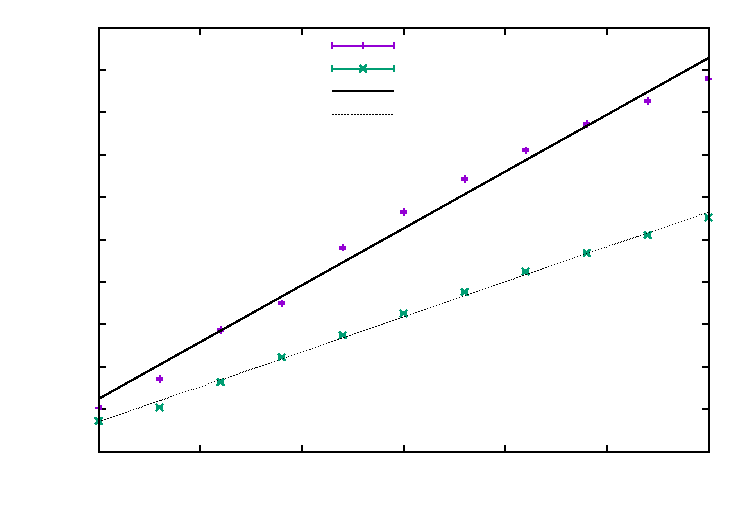
\includegraphics{AluSolar}}%
    \gplfronttext
  \end{picture}%
\endgroup

	\caption{Messwerte und Fit der Temperatur der beiden Aluplatten im Zeitverlauf.}
	\label{fig:aluSW}
\end{figure}


\newpage
\section{Erhitzen von Sand im Vergleich zu Wasser}
Da ertragreiche Solarkraftwerke per Definition in eher trockenen (am besten Wüstenregionen) stehen würden, ist die Frage nach der Energiespeicherung für die Nacht interessant.
Man könnte überlegen, den Wüstensand der Umgebung einfach aufzuhitzen, da es den in großer Menge gibt.
Allerdings stellte sich in unserem zweiten Versuch heraus, dass das Wasser die Wärme viel besser speichern kann, als der Sand.
Dies äußerte sich darin, dass die beiden Behälter, welche zu Beginn des Experimentes annähernd gleich warm waren und der selben Strahlungsleistung ausgesetzt waren schnell sehr unterschiedliche Temperaturen hatten.
Die Steigungen von \ref{fig:wassersand} betragen
\begin{align*}
	\left( \frac{\Delta T}{\Delta t} \right)_\text{Wasser}&=\SI{0.057(2)}{\kelvin \per \second}\\
	\left( \frac{\Delta T}{\Delta t} \right)_\text{Sand}&=\SI{0.180(6)}{\kelvin \per \second}
\end{align*}
woraus sich (da die gleichen Massen und Oberflächen vorhanden sind) ein Verhältnis der spezifischen Wärmespeicherkoeffizienten von
\begin{align*}
	\frac{c_\text{Wasser}}{c_\text{Sand}}=3.16
\end{align*}

Dies bedeutet, dass Wasser bei gleicher Temperaturerhöhung mehr als die dreifache Energiemenge aufnehmen kann.
Nimmt man die Literaturwerte nach\footnote{\spezWaerme}, so soll Wasser $c_\text{Wasser}=\SI{4.186}{\kelvin \per \second}$ und $q_\text{Sand}=\SI{0.835}{\kelvin \per \second}$ besitzen.
Dies würde einem Verhältnis von $5.01$ entsprechen.
Allerdings hängt die Konstante vom Sand mit Sicherheit von extrem vielen Faktoren wie Korngröße und Dichte ab.
Die starke Tendenz ist jedoch zu erkennen.

\begin{figure}[h]
	\centering
	% GNUPLOT: LaTeX picture with Postscript
\begingroup
  \makeatletter
  \providecommand\color[2][]{%
    \GenericError{(gnuplot) \space\space\space\@spaces}{%
      Package color not loaded in conjunction with
      terminal option `colourtext'%
    }{See the gnuplot documentation for explanation.%
    }{Either use 'blacktext' in gnuplot or load the package
      color.sty in LaTeX.}%
    \renewcommand\color[2][]{}%
  }%
  \providecommand\includegraphics[2][]{%
    \GenericError{(gnuplot) \space\space\space\@spaces}{%
      Package graphicx or graphics not loaded%
    }{See the gnuplot documentation for explanation.%
    }{The gnuplot epslatex terminal needs graphicx.sty or graphics.sty.}%
    \renewcommand\includegraphics[2][]{}%
  }%
  \providecommand\rotatebox[2]{#2}%
  \@ifundefined{ifGPcolor}{%
    \newif\ifGPcolor
    \GPcolortrue
  }{}%
  \@ifundefined{ifGPblacktext}{%
    \newif\ifGPblacktext
    \GPblacktexttrue
  }{}%
  % define a \g@addto@macro without @ in the name:
  \let\gplgaddtomacro\g@addto@macro
  % define empty templates for all commands taking text:
  \gdef\gplbacktext{}%
  \gdef\gplfronttext{}%
  \makeatother
  \ifGPblacktext
    % no textcolor at all
    \def\colorrgb#1{}%
    \def\colorgray#1{}%
  \else
    % gray or color?
    \ifGPcolor
      \def\colorrgb#1{\color[rgb]{#1}}%
      \def\colorgray#1{\color[gray]{#1}}%
      \expandafter\def\csname LTw\endcsname{\color{white}}%
      \expandafter\def\csname LTb\endcsname{\color{black}}%
      \expandafter\def\csname LTa\endcsname{\color{black}}%
      \expandafter\def\csname LT0\endcsname{\color[rgb]{1,0,0}}%
      \expandafter\def\csname LT1\endcsname{\color[rgb]{0,1,0}}%
      \expandafter\def\csname LT2\endcsname{\color[rgb]{0,0,1}}%
      \expandafter\def\csname LT3\endcsname{\color[rgb]{1,0,1}}%
      \expandafter\def\csname LT4\endcsname{\color[rgb]{0,1,1}}%
      \expandafter\def\csname LT5\endcsname{\color[rgb]{1,1,0}}%
      \expandafter\def\csname LT6\endcsname{\color[rgb]{0,0,0}}%
      \expandafter\def\csname LT7\endcsname{\color[rgb]{1,0.3,0}}%
      \expandafter\def\csname LT8\endcsname{\color[rgb]{0.5,0.5,0.5}}%
    \else
      % gray
      \def\colorrgb#1{\color{black}}%
      \def\colorgray#1{\color[gray]{#1}}%
      \expandafter\def\csname LTw\endcsname{\color{white}}%
      \expandafter\def\csname LTb\endcsname{\color{black}}%
      \expandafter\def\csname LTa\endcsname{\color{black}}%
      \expandafter\def\csname LT0\endcsname{\color{black}}%
      \expandafter\def\csname LT1\endcsname{\color{black}}%
      \expandafter\def\csname LT2\endcsname{\color{black}}%
      \expandafter\def\csname LT3\endcsname{\color{black}}%
      \expandafter\def\csname LT4\endcsname{\color{black}}%
      \expandafter\def\csname LT5\endcsname{\color{black}}%
      \expandafter\def\csname LT6\endcsname{\color{black}}%
      \expandafter\def\csname LT7\endcsname{\color{black}}%
      \expandafter\def\csname LT8\endcsname{\color{black}}%
    \fi
  \fi
    \setlength{\unitlength}{0.0500bp}%
    \ifx\gptboxheight\undefined%
      \newlength{\gptboxheight}%
      \newlength{\gptboxwidth}%
      \newsavebox{\gptboxtext}%
    \fi%
    \setlength{\fboxrule}{0.5pt}%
    \setlength{\fboxsep}{1pt}%
\begin{picture}(7200.00,5040.00)%
    \gplgaddtomacro\gplbacktext{%
      \csname LTb\endcsname%
      \put(682,704){\makebox(0,0)[r]{\strut{}$10$}}%
      \put(682,1286){\makebox(0,0)[r]{\strut{}$20$}}%
      \put(682,1867){\makebox(0,0)[r]{\strut{}$30$}}%
      \put(682,2449){\makebox(0,0)[r]{\strut{}$40$}}%
      \put(682,3030){\makebox(0,0)[r]{\strut{}$50$}}%
      \put(682,3612){\makebox(0,0)[r]{\strut{}$60$}}%
      \put(682,4193){\makebox(0,0)[r]{\strut{}$70$}}%
      \put(682,4775){\makebox(0,0)[r]{\strut{}$80$}}%
      \put(814,484){\makebox(0,0){\strut{}$0$}}%
      \put(1812,484){\makebox(0,0){\strut{}$50$}}%
      \put(2810,484){\makebox(0,0){\strut{}$100$}}%
      \put(3809,484){\makebox(0,0){\strut{}$150$}}%
      \put(4807,484){\makebox(0,0){\strut{}$200$}}%
      \put(5805,484){\makebox(0,0){\strut{}$250$}}%
      \put(6803,484){\makebox(0,0){\strut{}$300$}}%
    }%
    \gplgaddtomacro\gplfronttext{%
      \csname LTb\endcsname%
      \put(176,2739){\rotatebox{-270}{\makebox(0,0){\strut{}T [$\si\celsius$]}}}%
      \put(3808,154){\makebox(0,0){\strut{}Zeit [s]}}%
      \csname LTb\endcsname%
      \put(2794,4602){\makebox(0,0)[r]{\strut{}Wasser (Werte)}}%
      \csname LTb\endcsname%
      \put(2794,4382){\makebox(0,0)[r]{\strut{}Sand (Werte)}}%
      \csname LTb\endcsname%
      \put(2794,4162){\makebox(0,0)[r]{\strut{}Wasser (Fit)}}%
      \csname LTb\endcsname%
      \put(2794,3942){\makebox(0,0)[r]{\strut{}Sand (Fit)}}%
    }%
    \gplbacktext
    \put(0,0){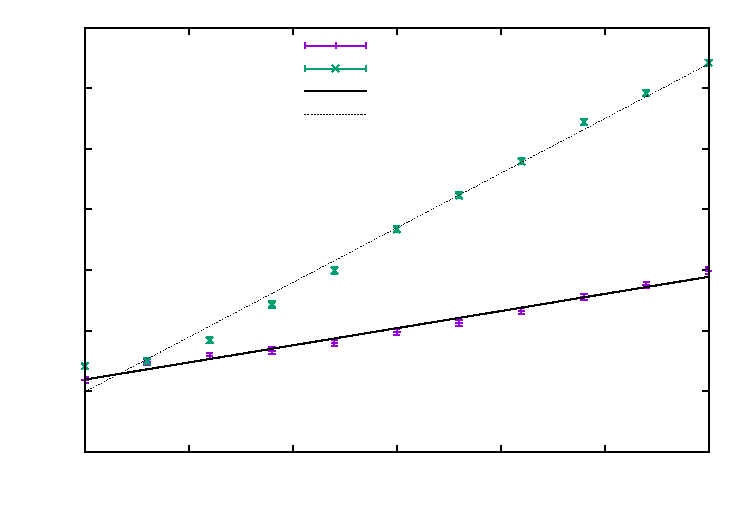
\includegraphics{WasserSandSolar}}%
    \gplfronttext
  \end{picture}%
\endgroup

	\caption{Temperaturverlauf von Wasser und Sand im Zeitverlauf, sowie der lineare Fit.}
	\label{fig:wassersand}
\end{figure}






\end{document}
